%===================================================%
%-->    Lab: AC Introduction and Voltage Divider <--%
%--> Author: Charles Edward Pax                  <--%
%-->   Date: 2006.01.31                          <--%
%===================================================%
% NOTE: The README file contains much more detailed descriptions of all the commands you might need.

\documentclass[11pt,onecolumn]{article}
% This sets the document type to be used to "article" and activates any desired style optioins.
% Options
% ====================
% Name		Description
% --------	-----------
% 10pt		Set font size to 10 points
% 11pt		Set font size to 11 points
% 12pt		Set font size to 12 points
% onecolumn	Set number of columns to one
% twocolumn	Set number of columns to two

\usepackage{color,graphics}
% Options
% ====================
% Name		Description
% --------	-----------
% color		Allows the inclusion of colors.
% graphics	Allows the inclusion of various graphics.
% pstricks	Allows many complex graphic functions such as circuit diagrams.

\begin{document}
% This command tells LaTeX to process the following commands as part of the document body.

\title{AC Introduction and Voltage Divider}
% This command defines the title of the report for use in the "\maketitle" command below.

\date{\today}
% This command defines the date for use in the "\maketitle" command below. You may manually type any date or use one of the following options.
% Options
% ====================
% Name		Description
% --------	-----------
% \today	Includes the date the documents is compiled

\author{Charles Edward Pax}
% This command defines the author's name for use in the "\maketitle" command below.

\maketitle
% This command includes the title, author name, and date in the final document.

%=====================%
%--> Sec: Abstract <--%
%=====================%
\abstract{This report demonstrates the author's knolwedge of the AC voltage divider, differentiator, and oscilloscope technique.}
% This command tells LaTeX to format the contained text in a way particular to the abstract. The abstract is a breif paragraph describing the purpose, methods, and results of the experiment.

%=========================%
%--> Sec: Introduction <--%
%=========================%
\section{Introduction}\label{sec:Introduction}
The AC voltage divider shown in figure \ref{fig:AC Voltage Divider} structurally similar to a DC voltage divider, where $Z_1$ and $Z_2$ are resistors, with the important difference begin that $Z_2$ is a capacitor. The $V_{out}$ in figure \ref{fig:AC Voltage Divider} is described by equation \ref{eq:AC Voltage Divider}

\begin{figure}
\begin{center}
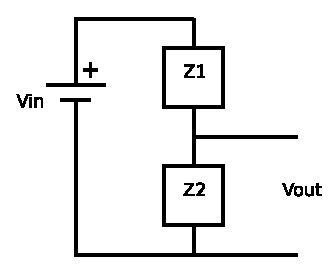
\includegraphics{Diagram1.eps}
\end{center}
\caption{AC voltage divider. $Z_1$ is a resistor and $Z_2$ is a capacitor.}\label{fig:AC Voltage Divider}
\end{figure}

\begin{equation}\label{eq:AC Voltage Divider}
V_{out} = V_{in} \frac{Z_2}{Z_1 + Z_2}
\end{equation}

%=================%
%--> Sec: Data <--%
%=================%
\section{Data}\label{sec:Data}
The circuit was assembled with R = 20 k$\Omega$ and C = 1000 pF.Because the impedance $Z_1$ depends on frequency, the output voltage $V_{out}$ also depends on frequency; angular frequency $\omega$ begin related to frequency $f$ by $\omega = 2 \pi f$ \cite{DoPb}.

The sinusoidal input voltage was used while measuring the dependence of the magnitude and phase of $V_{out}$ relative to $V_{in}$. The results of these measurements are plotted with their theoretical values in figures \ref{fig:plot01} and \ref{fig:plot02} respectivly. Measurements were taken at various frequencies ranging from 100 Hz to 1 MHz.
\begin{figure}
\input{plot01}
\caption{The dependence of the magnitude and phase of $V_{out}$ relative to $V_{in}$ experimental and theoretical.}\label{fig:plot01}
\end{figure}

\begin{figure}
\input{plot02}
\caption{Some caption.}\label{fig:plot02}
\end{figure}


The exponential decay time dependence, a function generator was used to create a square wave pulse. Using equation \ref{eq:N} the exponential decay constant $\lambda$ can be found.
\begin{equation}\label{eq:N}
N = N_0 e^{- \lambda t}
\end{equation}
For $t = 0$,
\begin{displaymath}
\lambda = \mathrm{ln}\left(\frac{N}{N_0} \frac{-1}{t}\right) = 45647.6
\end{displaymath}
The decay calculated from $C$ and $R$ is plotted along with the measured values in figure \ref{fig:plot03}.
\begin{figure}
\input{plot03}
\caption{Some caption.}\label{fig:plot03}
\end{figure}

%=======================%
%--> Sec: Discussion <--%
%=======================%
\section{Discussion \& Analysis}\label{sec:Discussion}
The circuit in figure \ref{fig:AC Voltage Divider} can also be used as a differentiator. The function generator was used to generate a triangular waveform. The output and input voltages were plotted on the oscilloscope screen as a function of time. The square wave $V_{out}$ is suprisingly similar to the proper differentiated values of the triangular wave. $V_{out}$ is positive or negative when the triangular wave has a positive or negative slope respectivly. The amplitude of the square wave is also what one would expect given the amplitude of $V_{in}$.

%=========================%
%--> Sec: Bibliography <--%
%=========================%
\begin{thebibliography}{9}
% This command tells LaTeX to create "References" section containing all the references that are not commented out. Be sure to uncomment all the references which you use and add those that are not currently listed.
\bibitem{DoPb} Rutgers University, Physics 327, {\em AC Introduction and Voltage Divider} January 25, 2006.
\end{thebibliography}

\end{document}

%=================%
%--> Templates <--%
%=================%
% This section contains templates for commonly used environments. This section will not appear in you final document as it come after the "\end{document}" command above.

% Equation template
\begin{equation}\label{eq:eqLabel}
math = good^2
\end{equation}

% Figure template
\begin{figure}
\input{graphicFile}
\caption{This is the caption. It should include a short description of the figure.}\label{fig:figureLabel}
\end{figure}
